%=======================================================================
%  Informe Técnico — Hito 1 — Proyecto Final Integrador
%  Robótica IMT-342 — Grupo VEVAS
%  Compilar:  pdflatex informe.tex  (dos veces, por el índice)
%=======================================================================
\documentclass[11pt,a4paper]{article}

\usepackage[utf8]{inputenc}
\usepackage[T1]{fontenc}
%babel no disponible en este sistema
\usepackage{charter}
\usepackage[a4paper,margin=2.5cm,headheight=14pt]{geometry}
\usepackage{amsmath,amssymb,amsfonts}
\usepackage{graphicx}
\usepackage{booktabs}
\usepackage{longtable}
\usepackage{array}
\usepackage{xcolor}
\usepackage{listings}
\usepackage{fancyhdr}
\usepackage{caption}
\usepackage{subcaption}
\usepackage{enumitem}
\usepackage{tikz}
\usetikzlibrary{shapes.geometric,arrows.meta,positioning,calc}
\usepackage[hidelinks]{hyperref}

%---------------------------------------------------- colores y estilo
\definecolor{naranja}{HTML}{D2601A}
\definecolor{oscuro}{HTML}{1F2A33}
\definecolor{gris}{HTML}{5A6672}
\definecolor{fondocodigo}{HTML}{F5F6F7}
\definecolor{comentario}{HTML}{6A8759}
\definecolor{clave}{HTML}{9B2D30}

\lstset{
  basicstyle=\ttfamily\scriptsize,
  backgroundcolor=\color{fondocodigo},
  keywordstyle=\color{clave}\bfseries,
  commentstyle=\color{comentario}\itshape,
  stringstyle=\color{naranja},
  numbers=left, numberstyle=\tiny\color{gris}, numbersep=8pt,
  frame=leftline, framerule=1.2pt, rulecolor=\color{naranja},
  breaklines=true, breakatwhitespace=false,
  showstringspaces=false, tabsize=4,
  xleftmargin=14pt, framexleftmargin=14pt,
  captionpos=b, literate={á}{{\'a}}1 {é}{{\'e}}1 {í}{{\'i}}1
    {ó}{{\'o}}1 {ú}{{\'u}}1 {ñ}{{\~n}}1 {Á}{{\'A}}1 {É}{{\'E}}1
    {Í}{{\'I}}1 {Ó}{{\'O}}1 {Ú}{{\'U}}1 {Ñ}{{\~N}}1 {¿}{{?`}}1 {¡}{{!`}}1
}

\pagestyle{fancy}
\fancyhf{}
\lhead{\small\color{gris}Hito 1 — Gemelo Digital ABB IRB 120}
\rhead{\small\color{gris}Grupo VEVAS}
\cfoot{\small\color{gris}\thepage}
\renewcommand{\headrulewidth}{0.4pt}

\captionsetup{font=small,labelfont={bf,color=naranja}}

%---------------------------------------------------- macros
\newcommand{\T}[2]{{}^{#1}\mathbf{T}_{#2}}
\newcommand{\R}[2]{{}^{#1}\mathbf{R}_{#2}}
\newcommand{\mat}[1]{\mathbf{#1}}
\newcommand{\Rz}{\mathrm{Rot}(z,\cdot)}

\newenvironment{nota}
  {\begin{quote}\small\color{oscuro}\rule{2pt}{\baselineskip}\hspace{6pt}\ignorespaces}
  {\end{quote}}

%=======================================================================
\begin{document}

%---------------------------------------------------------- PORTADA
\begin{titlepage}
\centering
\vspace*{1.2cm}

{\color{gris}\large UNIVERSIDAD CATÓLICA BOLIVIANA ``SAN PABLO''}\\[2pt]
{\color{gris} Unidad Académica Regional Tarija \quad|\quad Ingeniería Mecatrónica}

\vspace{2.2cm}

{\color{naranja}\rule{\textwidth}{2pt}}
\vspace{0.7cm}

{\Huge\bfseries Gemelo Digital Cinemático\\[6pt] del Manipulador ABB IRB 120\par}

\vspace{0.7cm}
{\large\itshape Del modelo Denavit--Hartenberg a la descripción URDF\\
validada en ROS 2 con error vectorial $\Delta E < 10^{-6}$~m\par}

\vspace{0.5cm}
{\color{naranja}\rule{\textwidth}{2pt}}

\vspace{1.6cm}

{\large\bfseries Hito 1 — Proyecto Final Integrador\par}
\vspace{4pt}
{\large Celda de Manufactura Flexible Inteligente\par}

\vspace{2.2cm}

\begin{minipage}{0.8\textwidth}
\centering
{\large\bfseries GRUPO VEVAS}\\[10pt]
{\large
Susann Baldiviezo C.\\[3pt]
Florencia Frigerio\\[3pt]
Alejandro Bejarano R.\\[3pt]
Benjamín Soruco G.\\
}
\end{minipage}

\vspace{2.0cm}

{\large \textbf{Docente:} M.Sc. Ing. Bernardo Quiroga Turdera\par}
\vspace{4pt}
{\large Robótica — IMT-342 \quad|\quad Gestión II-2026\par}

\vfill
{\color{gris}\small Tarija, Bolivia}
\end{titlepage}

%---------------------------------------------------------- RESUMEN
\section*{Resumen}
\addcontentsline{toc}{section}{Resumen}

Este informe documenta la construcción y validación del gemelo digital
cinemático del manipulador industrial ABB IRB 120 de seis grados de
libertad, correspondiente al Hito 1 del Proyecto Final Integrador de la
asignatura Robótica (IMT-342).

El trabajo parte de la parametrización de Denavit--Hartenberg del
manipulador, deriva analíticamente su cinemática directa y construye a
partir de ella una descripción URDF para ROS 2. La contribución central
del grupo consiste en que los orígenes del URDF no fueron ajustados
visualmente, sino \emph{derivados} mediante una relación algebraica
cerrada entre ambos formalismos:
\[
\mat{O}_i \;=\; \mat{B}_{i-1}\,\mathrm{Rot}(z,\theta_{\mathrm{off},i}),
\qquad
\mat{B}_i = \mathrm{Tras}(z,d_i)\,\mathrm{Tras}(x,a_i)\,\mathrm{Rot}(x,\alpha_i).
\]

La equivalencia entre el modelo matemático y el modelo computacional se
verificó mediante tres pruebas independientes: la predicción de la pose
en la configuración cero por suma directa de cotas del manual del
fabricante, la comparación entre una descripción URDF escrita
manualmente y otra generada programáticamente, y un barrido aleatorio
del espacio articular contrastando el árbol de transformadas de ROS
contra la función analítica.

El resultado principal es un error posicional máximo de
$2{,}459\times10^{-10}$~m sobre 501 configuraciones válidas, cuatro mil
veces por debajo del umbral de $10^{-6}$~m exigido por el hito, con
validación simultánea de la orientación. El informe documenta además
tres discrepancias detectadas durante el desarrollo, dos de ellas con
errores superiores a un metro, junto con su diagnóstico y corrección.

\vspace{6pt}
\noindent\textbf{Palabras clave:} Denavit--Hartenberg, cinemática
directa, URDF, ROS 2, SE(3), gemelo digital, ABB IRB 120.

\vspace{10pt}
\noindent\textbf{Repositorio:}
\url{https://github.com/FlorenciaFrigerio/pfi-hito1-vevas}

\newpage
\tableofcontents
\newpage

%=======================================================================
\section{Introducción}

\subsection{Contexto}

El Proyecto Final Integrador de la asignatura plantea el desarrollo de
una celda de manufactura flexible con clasificación y paletizado
autónomo por visión artificial sobre un manipulador ABB IRB 120. El
proyecto se estructura en cuatro hitos sucesivos, de los cuales el
primero —objeto de este informe— corresponde a la construcción del
modelo cinemático directo y su representación computacional.

El Hito 1 no es un ejercicio aislado: el modelo que aquí se valida es la
entrada directa del resolvedor de cinemática inversa por desacoplamiento
de Pieper que se implementará en el Hito 2. Un error en la asignación de
ejes en esta etapa no se manifiesta necesariamente ahora, pero invalida
todo el trabajo posterior.

\subsection{Planteamiento del problema}

Un manipulador industrial es un objeto físico; un programa de control es
un objeto computacional. Entre ambos debe existir una descripción
matemática que sea a la vez fiel a la geometría real y manipulable
algorítmicamente.

El problema concreto de este hito puede enunciarse así:

\begin{nota}
Dado el manipulador ABB IRB 120 con sus cotas geométricas de fábrica,
construir una descripción URDF cuyo árbol de transformadas coincida, para
cualquier configuración articular admisible, con la cinemática directa
derivada analíticamente de la convención Denavit--Hartenberg, y demostrar
numéricamente esa coincidencia.
\end{nota}

La dificultad no está en obtener \emph{alguna} descripción que se vea
correcta en un visualizador. Está en garantizar que las dos
representaciones —la analítica y la computacional— son el mismo operador
del grupo especial euclídeo $SE(3)$, y en poder demostrarlo.

\subsection{Objetivos}

\subsubsection*{Objetivo general}

Construir y validar el gemelo digital cinemático del ABB IRB 120,
estableciendo la equivalencia demostrable entre su modelo matemático
Denavit--Hartenberg y su descripción URDF ejecutable en ROS 2.

\subsubsection*{Objetivos específicos}

\begin{enumerate}[label=\textbf{O\arabic*.},leftmargin=*]
\item Asignar los sistemas de coordenadas locales según la convención
      Denavit--Hartenberg estándar e identificar los desplazamientos
      constantes (\emph{offsets}) de las juntas.
\item Derivar la cinemática directa $\T{0}{6}(\mat{q})$ e implementarla
      desde primeros principios, sin recurrir a bibliotecas de robótica.
\item Establecer una relación algebraica cerrada entre los parámetros
      D--H y los atributos \texttt{origin} del formato URDF.
\item Construir la descripción URDF y validar su sintaxis y su árbol
      cinemático.
\item Demostrar la validez del modelo mediante una matriz de pruebas con
      error vectorial inferior a $10^{-6}$~m.
\item Mantener un historial de versiones trazable que refleje el proceso
      real de trabajo.
\end{enumerate}

\subsection{Alcance y limitaciones}

Este hito cubre exclusivamente la cinemática \emph{directa} y su
representación. Quedan fuera del alcance la cinemática inversa (Hito 2),
la calibración mano-ojo y la segmentación por visión (Hito 3), y la
integración física con el controlador IRC5 (Hito 4).

La geometría visual se implementó mediante primitivas geométricas
dimensionadas a partir de la propia tabla D--H, en lugar de mallas
importadas. Esta decisión se justifica en la sección~\ref{sec:visual}.

%=======================================================================
\section{Marco teórico}

\subsection{El grupo especial euclídeo \texorpdfstring{$SE(3)$}{SE(3)}}

La pose de un cuerpo rígido en el espacio queda completamente
determinada por su posición y su orientación. Matemáticamente se
representa mediante una transformación homogénea
\begin{equation}
\mat{T} =
\begin{bmatrix}
\mat{R} & \mat{p}\\
\mat{0}^{\top} & 1
\end{bmatrix}
\in SE(3),
\qquad
\mat{R}\in SO(3),\;\; \mat{p}\in\mathbb{R}^3,
\label{eq:se3}
\end{equation}
donde $\mat{R}$ es una matriz de rotación $3\times3$ y $\mat{p}$ el
vector de traslación.

El conjunto $SO(3)$ de matrices de rotación se caracteriza por dos
propiedades que se utilizarán repetidamente:
\begin{equation}
\mat{R}^{\top}\mat{R} = \mat{I}
\quad\Longrightarrow\quad
\mat{R}^{-1} = \mat{R}^{\top},
\qquad
\det(\mat{R}) = +1.
\label{eq:so3}
\end{equation}

La ortogonalidad tiene una consecuencia práctica importante: la inversa
de una transformación homogénea se obtiene sin invertir numéricamente
una matriz $4\times4$,
\begin{equation}
\mat{T}^{-1} =
\begin{bmatrix}
\mat{R}^{\top} & -\mat{R}^{\top}\mat{p}\\
\mat{0}^{\top} & 1
\end{bmatrix},
\label{eq:inversa}
\end{equation}
expresión exacta que no acumula error numérico y resulta
sustancialmente más rápida.

\begin{nota}
$SE(3)$ \textbf{no es conmutativo}. En general
$\mat{T}_1\mat{T}_2 \neq \mat{T}_2\mat{T}_1$: rotar y luego trasladar no
produce el mismo resultado que trasladar y luego rotar. Esta propiedad
determina el orden estricto de las operaciones en la
sección~\ref{sec:elemental} y es la razón por la cual la conversión
D--H~$\to$~URDF requiere una factorización cuidadosa.
\end{nota}

\subsection{Composición de transformaciones}

Si $\T{0}{1}$ describe el marco 1 respecto del marco 0, y $\T{1}{2}$
describe el marco 2 respecto del marco 1, entonces
\begin{equation}
\T{0}{2} = \T{0}{1}\,\T{1}{2}.
\end{equation}

La \emph{post}-multiplicación corresponde a transformaciones expresadas
en el marco móvil: cada nueva transformación se aplica respecto del
sistema recién obtenido, no del sistema fijo. Esta es la convención que
se emplea en todo el trabajo.

%=======================================================================
\section{El manipulador ABB IRB 120}

\subsection{Morfología}

El IRB 120 es un manipulador antropomórfico de cadena cinemática abierta
con seis juntas de revolución. Sus características relevantes se
resumen en el cuadro~\ref{tab:specs}.

\begin{table}[h]
\centering
\caption{Características del ABB IRB 120 según manual del fabricante}
\label{tab:specs}
\small
\begin{tabular}{@{}ll@{}}
\toprule
\textbf{Característica} & \textbf{Valor} \\
\midrule
Grados de libertad & 6 (todas de revolución) \\
Alcance máximo & 580 mm \\
Carga útil & 3 kg \\
Repetibilidad de posición & $\pm$0,01 mm \\
Masa & 25 kg \\
Configuración de muñeca & Esférica (ejes 4, 5 y 6 concurrentes) \\
Controlador & IRC5 Compact \\
\bottomrule
\end{tabular}
\end{table}

\begin{figure}[h]
\centering
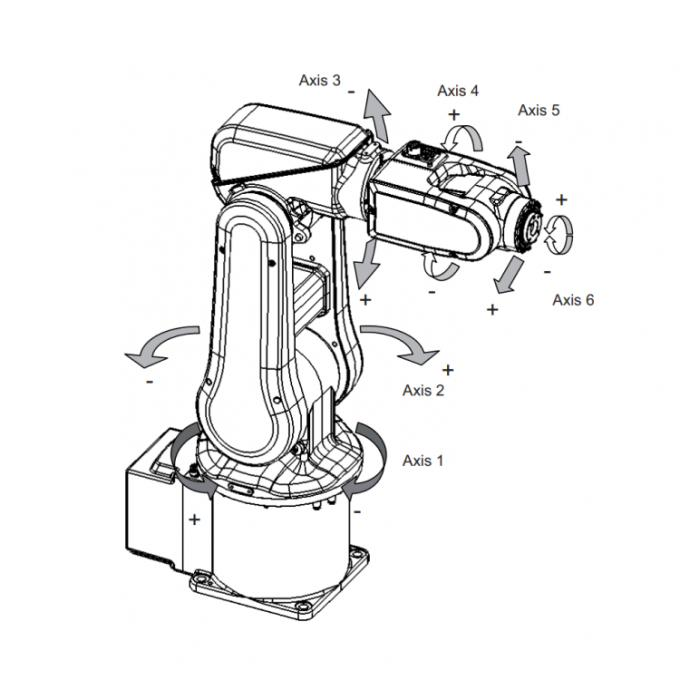
\includegraphics[width=0.52\textwidth]{img/abb_irb_120.png}
\caption{Manipulador ABB IRB 120 y disposición de sus seis juntas de
revolución.}
\label{fig:robot}
\end{figure}

\subsection{La muñeca esférica y su consecuencia matemática}

El dato morfológico más relevante para el modelado no aparece en las
especificaciones comerciales: las juntas 4, 5 y 6 conforman una
\textbf{muñeca esférica}, es decir, sus tres ejes de rotación se cortan
en un único punto del espacio.

Geométricamente esto implica $a_4 = a_5 = 0$ en la parametrización
D--H. La consecuencia matemática es el \emph{desacoplamiento
cinemático}: la posición del centro de muñeca depende exclusivamente de
$q_1, q_2, q_3$, mientras que la orientación del efector depende
exclusivamente de $q_4, q_5, q_6$.

\begin{nota}
Este desacoplamiento es lo que permite resolver el problema cinemático
inverso —seis ecuaciones con seis incógnitas acopladas— como dos
subproblemas independientes de tres incógnitas cada uno. Es el
fundamento del método de Pieper que se implementará en el Hito 2. Por
esa razón, aunque este hito trate únicamente de cinemática directa, la
correcta asignación de los ejes de la muñeca es crítica.
\end{nota}

%=======================================================================
\section{Parametrización Denavit--Hartenberg}

\subsection{Justificación de la convención}

Una transformación arbitraria entre dos marcos en $SE(3)$ requiere seis
parámetros independientes: tres de traslación y tres de rotación. Para
un manipulador de seis eslabones esto significa $6\times6 = 36$
parámetros que deberían medirse, documentarse y mantenerse consistentes
entre sí. Peor aún, dos ingenieros distintos elegirían marcos distintos
y obtendrían descripciones incomparables.

La convención Denavit--Hartenberg resuelve el problema restringiendo la
libertad de elección de los marcos. Impone dos condiciones:

\begin{enumerate}[label=(\roman*),leftmargin=*]
\item el eje $x_i$ debe ser perpendicular al eje $z_{i-1}$;
\item el eje $x_i$ debe intersecar al eje $z_{i-1}$.
\end{enumerate}

Cada condición elimina un grado de libertad de la descripción. De los
seis parámetros originales quedan cuatro:
\begin{equation}
\theta_i,\; d_i,\; a_i,\; \alpha_i.
\end{equation}

El total desciende a 24 parámetros, de los cuales sólo seis —los
$\theta_i$ en un manipulador de juntas rotacionales— son variables.

\begin{nota}
La convención no es una preferencia de estilo: es una \emph{reducción de
dimensionalidad} del espacio de descripciones posibles que convierte la
parametrización en canónica y, por tanto, reproducible.
\end{nota}

\subsection{Reglas de asignación de ejes}

La asignación de marcos es el único paso no mecánico del procedimiento;
todo lo demás se deduce de ella.

\begin{enumerate}[label=\textbf{R\arabic*.},leftmargin=*]
\item \textbf{Eje $z_i$:} se alinea con el eje de rotación de la junta
      $i+1$. Es el eje sobre el que actúa la variable $q_{i+1}$.
\item \textbf{Eje $x_i$:} se dispone a lo largo de la perpendicular
      común entre $z_{i-1}$ y $z_i$, orientado de $z_{i-1}$ hacia $z_i$.
\item \textbf{Origen $O_i$:} en la intersección de $x_i$ con $z_i$.
\item \textbf{Eje $y_i$:} se completa por la regla de la mano derecha,
      $y_i = z_i \times x_i$. Nunca se elige libremente.
\end{enumerate}

\subsubsection*{Casos degenerados presentes en el IRB 120}

\textbf{Ejes paralelos ($z_{i-1} \parallel z_i$).} Ocurre entre las
juntas 2 y 3. Cuando dos ejes son paralelos existen infinitas
perpendiculares comunes, de modo que la regla R2 no determina
unívocamente $x_i$. Por convención se elige la perpendicular que anula
$d_i$.

\textbf{Ejes concurrentes ($z_{i-1} \cap z_i \neq \emptyset$).} Ocurre
en la muñeca. La perpendicular común degenera a un punto y $a_i = 0$.

\begin{nota}
La ambigüedad del caso de ejes paralelos explica por qué distintas
publicaciones proporcionan tablas D--H diferentes para el mismo
manipulador. Este trabajo adopta la parametrización de Truc y Lam
(2020), y lo declara explícitamente, tal como se recomienda en la
literatura para garantizar reproducibilidad.
\end{nota}

\subsection{La matriz de transformación elemental}
\label{sec:elemental}

El paso del marco $i-1$ al marco $i$ se compone siempre de la misma
secuencia de cuatro movimientos elementales, en orden estricto:

\begin{equation}
\boxed{\;
\T{i-1}{i} =
\mathrm{Rot}(z,\theta_i)\;
\mathrm{Tras}(z,d_i)\;
\mathrm{Tras}(x,a_i)\;
\mathrm{Rot}(x,\alpha_i)
\;}
\label{eq:elemental}
\end{equation}

La interpretación física de cada factor es la siguiente:

\begin{center}
\small
\begin{tabular}{@{}ll@{}}
\toprule
\textbf{Factor} & \textbf{Significado} \\
\midrule
$\mathrm{Rot}(z,\theta_i)$ & Gira el marco hasta alinear $x_{i-1}$ con $x_i$. Es la variable de junta. \\
$\mathrm{Tras}(z,d_i)$ & Desliza sobre $z_{i-1}$ hasta la altura de la perpendicular común. \\
$\mathrm{Tras}(x,a_i)$ & Recorre la perpendicular común: la longitud real del eslabón. \\
$\mathrm{Rot}(x,\alpha_i)$ & Gira para alinear $z_{i-1}$ con $z_i$: el torcimiento del eslabón. \\
\bottomrule
\end{tabular}
\end{center}

\subsubsection*{Desarrollo analítico}

Expandiendo el producto~\eqref{eq:elemental}:

\begin{align}
\mathrm{Rot}(z,\theta) &=
\begin{bmatrix}
c\theta & -s\theta & 0 & 0\\
s\theta & c\theta & 0 & 0\\
0&0&1&0\\ 0&0&0&1
\end{bmatrix},
&
\mathrm{Tras}(z,d) &=
\begin{bmatrix}
1&0&0&0\\ 0&1&0&0\\ 0&0&1&d\\ 0&0&0&1
\end{bmatrix},\\[6pt]
\mathrm{Tras}(x,a) &=
\begin{bmatrix}
1&0&0&a\\ 0&1&0&0\\ 0&0&1&0\\ 0&0&0&1
\end{bmatrix},
&
\mathrm{Rot}(x,\alpha) &=
\begin{bmatrix}
1&0&0&0\\
0& c\alpha & -s\alpha & 0\\
0& s\alpha & c\alpha & 0\\
0&0&0&1
\end{bmatrix},
\end{align}

donde $c\theta \equiv \cos\theta$ y $s\theta \equiv \sin\theta$.
El producto resulta:

\begin{equation}
\boxed{\;
\T{i-1}{i} =
\begin{bmatrix}
c\theta_i & -s\theta_i c\alpha_i & \phantom{-}s\theta_i s\alpha_i & a_i c\theta_i\\
s\theta_i & \phantom{-}c\theta_i c\alpha_i & -c\theta_i s\alpha_i & a_i s\theta_i\\
0 & s\alpha_i & c\alpha_i & d_i\\
0 & 0 & 0 & 1
\end{bmatrix}
\;}
\label{eq:dh}
\end{equation}

Esta matriz se implementa directamente en el código, evitando cuatro
productos matriciales por junta en cada evaluación.

\begin{nota}
Obsérvese un detalle que se utilizará más adelante: las traslaciones
puras \emph{sí} conmutan entre sí, de modo que
$\mathrm{Tras}(z,d)\,\mathrm{Tras}(x,a)$ colapsa al vector
$(a, 0, d)$ expresado en el marco padre. Lo que no conmuta es la
rotación con la traslación.
\end{nota}

\subsection{Tabla D--H del ABB IRB 120}

\begin{figure}[h]
\centering
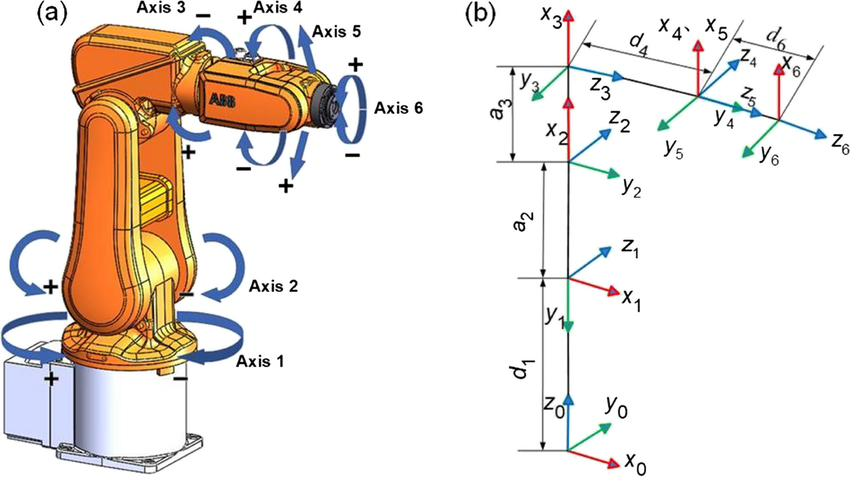
\includegraphics[width=0.62\textwidth]{img/dh_abb_irb_120.png}
\caption{Asignación de sistemas de coordenadas según la convención
Denavit--Hartenberg estándar sobre el ABB IRB 120.}
\label{fig:ejes}
\end{figure}

\begin{table}[h]
\centering
\caption{Parámetros Denavit--Hartenberg del ABB IRB 120
(parametrización de Truc y Lam, 2020), contrastados con las cotas del
manual técnico del fabricante}
\label{tab:dh}
\small
\begin{tabular}{@{}cccccl@{}}
\toprule
$i$ & $\theta_i$ & $d_i$ [m] & $a_i$ [m] & $\alpha_i$ [rad] & \textbf{Interpretación física} \\
\midrule
1 & $q_1$            & 0,290 & 0,000 & $-\pi/2$ & Altura de la columna base \\
2 & $q_2 - \pi/2$    & 0,000 & 0,270 & $0$      & Brazo; ejes $z_1 \parallel z_2$ \\
3 & $q_3$            & 0,000 & 0,070 & $-\pi/2$ & Codo; offset lateral corto \\
4 & $q_4$            & 0,302 & 0,000 & $+\pi/2$ & Antebrazo hacia la muñeca \\
5 & $q_5$            & 0,000 & 0,000 & $-\pi/2$ & Ejes concurrentes ($a_5=d_5=0$) \\
6 & $q_6$            & 0,072 & 0,000 & $0$      & Brida de salida (\texttt{tool0}) \\
\bottomrule
\end{tabular}
\end{table}

\subsection{Límites articulares}

Los límites del manual se expresan en grados y deben convertirse a
radianes para el archivo URDF. El cuadro~\ref{tab:limites} recoge la
conversión.

\begin{table}[h]
\centering
\caption{Límites articulares del ABB IRB 120}
\label{tab:limites}
\small
\begin{tabular}{@{}ccccc@{}}
\toprule
\textbf{Junta} & \textbf{Rango [grados]} & \textbf{Rango [rad]} & \textbf{Par [N$\cdot$m]} & \textbf{Vel. [rad/s]} \\
\midrule
J1 & $\pm165$ & $\pm2{,}879793$ & 42,0 & 4,36 \\
J2 & $\pm110$ & $\pm1{,}919862$ & 42,0 & 4,36 \\
J3 & $-110$ / $+70$ & $-1{,}919862$ / $+1{,}221730$ & 22,0 & 5,24 \\
J4 & $\pm160$ & $\pm2{,}792527$ & 5,0 & 5,58 \\
J5 & $\pm120$ & $\pm2{,}094395$ & 5,0 & 5,58 \\
J6 & $\pm400$ & $\pm6{,}981317$ & 3,0 & 7,33 \\
\bottomrule
\end{tabular}
\end{table}

\begin{nota}
La junta J3 es la \textbf{única asimétrica} del manipulador
($-110^\circ$ / $+70^\circ$), debido a la interferencia mecánica del
codo con el cuerpo del robot. Este detalle se pierde fácilmente al
transcribir la tabla y produce un modelo que admite configuraciones
físicamente imposibles.

Obsérvese además que escribir el valor en grados dentro del URDF
—por ejemplo \texttt{110} en lugar de \texttt{1.9199}— otorgaría al
modelo un recorrido de diecisiete vueltas completas.
\end{nota}

\subsection{El desplazamiento constante \texorpdfstring{$\theta_2 = q_2 - \pi/2$}{theta2}}
\label{sec:offset}

El segundo renglón de la tabla~\ref{tab:dh} contiene un término
constante que merece tratamiento aparte, por ser la fuente de error más
frecuente en el modelado de este manipulador.

Existen dos definiciones distintas de ``configuración cero'' que no
coinciden:

\begin{description}[leftmargin=*,style=nextline]
\item[Cero mecánico del fabricante.] $q_2 = 0$ corresponde a la postura
de calibración de ABB, con el brazo apuntando verticalmente hacia
arriba. Es el valor que indica el FlexPendant del controlador.
\item[Cero matemático de D--H.] $\theta_2 = 0$ exige, por la regla R2,
que $x_1$ y $x_2$ sean paralelos. Con los ejes asignados según la
convención, esto ocurre con el brazo en posición horizontal.
\end{description}

La diferencia entre ambas definiciones es exactamente $\pi/2$ radianes.
El desplazamiento constante reconcilia las dos referencias:
\begin{equation}
\theta_2 = q_2 - \frac{\pi}{2}.
\end{equation}

\begin{nota}
\textbf{El offset es una constante aditiva, no una variable.} Debe
codificarse una única vez dentro de la transformación y jamás sumarse en
el mensaje de estado articular. De omitirse, el manipulador aparece
rotado $90^\circ$ en el visualizador y el error respecto de la
cinemática analítica salta del orden de $10^{-10}$~m a
aproximadamente $0{,}3$~m.
\end{nota}

%=======================================================================
\section{Cinemática directa}

\subsection{Formulación}

La cinemática directa se obtiene encadenando las seis transformaciones
elementales:
\begin{equation}
\T{0}{6}(\mat{q}) = \prod_{i=1}^{6} \T{i-1}{i}(q_i)
= \T{0}{1}\,\T{1}{2}\,\T{2}{3}\,\T{3}{4}\,\T{4}{5}\,\T{5}{6}.
\label{eq:fk}
\end{equation}

El resultado es una matriz de $SE(3)$ que contiene simultáneamente la
posición y la orientación del efector respecto de la base.

\begin{nota}
El problema cinemático directo admite \textbf{siempre solución única}:
dada una configuración articular, existe una y sólo una pose del
efector. Es el problema inverso —objeto del Hito 2— el que puede
presentar cero, ocho o infinitas soluciones.
\end{nota}

\subsection{Evaluación en la configuración cero}

Evaluando~\eqref{eq:fk} en $\mat{q} = \mat{0}$:

\begin{equation}
\T{0}{6}(\mat{0}) =
\begin{bmatrix}
0 & 0 & 1 & 0{,}374\\
0 & -1 & 0 & 0{,}000\\
1 & 0 & 0 & 0{,}630\\
0 & 0 & 0 & 1
\end{bmatrix}
\end{equation}

de donde
\begin{equation}
\mat{p}(\mat{0}) = \begin{bmatrix}0{,}374 & 0{,}000 & 0{,}630\end{bmatrix}^{\top}\,\mathrm{m}.
\end{equation}

La matriz de rotación resultante indica que el eje $z$ de la brida
apunta en la dirección $x$ de la base: el efector mira hacia adelante,
horizontalmente, coherente con un brazo extendido. Se verifica
$\det(\mat{R}) = +1$, confirmando que se trata de una rotación propia.

\subsection{Verificación de cierre}
\label{sec:cierre}

La configuración cero permite un control de consistencia notable: la
pose puede predecirse \emph{sin multiplicar una sola matriz}, sumando
directamente las cotas del manual del fabricante.

\begin{align}
x &= d_4 + d_6 = 0{,}302 + 0{,}072 = 0{,}374\;\mathrm{m},\\
z &= d_1 + a_2 + a_3 = 0{,}290 + 0{,}270 + 0{,}070 = 0{,}630\;\mathrm{m},\\
y &= 0.
\end{align}

El error entre la predicción por suma de cotas y el producto matricial
es de $2{,}08\times10^{-18}$~m, es decir, nulo dentro de la precisión de
punto flotante de doble precisión.

\subsubsection*{Por qué es lícito sumar}

En general las longitudes de los eslabones \emph{no} pueden sumarse:
cada eslabón se encuentra rotado respecto del anterior y es necesario
componer matrices. Sin embargo, en $\mat{q} = \mat{0}$ el manipulador
adopta una configuración en la que los eslabones se alinean con
únicamente dos direcciones del marco base: primero apilan verticalmente
sobre $z$, luego se extienden horizontalmente sobre $x$. No aparecen
componentes cruzadas.

La figura~\ref{fig:origenes} muestra los orígenes de los marcos
intermedios, calculados truncando el producto~\eqref{eq:fk}.

\begin{figure}[h]
\centering
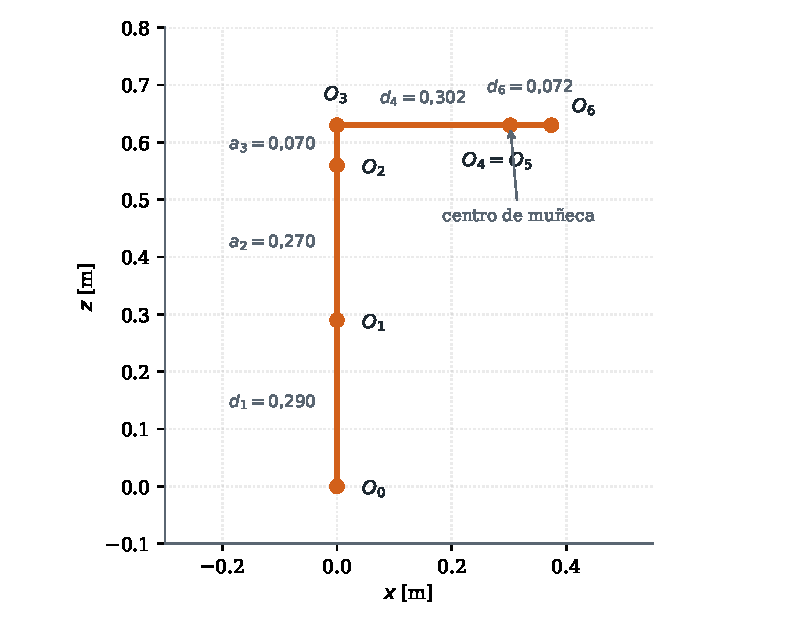
\includegraphics[width=0.66\textwidth]{img/origenes.pdf}
\caption{Orígenes de los sistemas de coordenadas en la configuración
cero, proyectados sobre el plano $xz$. Cada segmento corresponde
exactamente a una cota del manual del fabricante. Los marcos 4 y 5
coinciden en el espacio: es el centro de la muñeca esférica.}
\label{fig:origenes}
\end{figure}

\begin{table}[h]
\centering
\caption{Orígenes de los marcos intermedios en $\mat{q}=\mat{0}$}
\label{tab:origenes}
\small
\begin{tabular}{@{}cccl@{}}
\toprule
\textbf{Marco} & $x$ [m] & $z$ [m] & \textbf{Incremento respecto del anterior} \\
\midrule
$O_1$ & 0,00000 & 0,29000 & $+d_1 = 0{,}290$ \\
$O_2$ & 0,00000 & 0,56000 & $+a_2 = 0{,}270$ \\
$O_3$ & 0,00000 & 0,63000 & $+a_3 = 0{,}070$ \\
$O_4$ & 0,30200 & 0,63000 & $+d_4 = 0{,}302$ (cambia de eje) \\
$O_5$ & 0,30200 & 0,63000 & sin traslación: $a_5 = d_5 = 0$ \\
$O_6$ & 0,37400 & 0,63000 & $+d_6 = 0{,}072$ \\
\bottomrule
\end{tabular}
\end{table}

\begin{nota}
\textbf{Por qué $a_2$ y $a_3$ incrementan la altura.} En la convención
D--H el parámetro $a$ representa una traslación a lo largo del eje $x$
\emph{local}, no del marco base. Tras aplicar $\alpha_1 = -\pi/2$ en la
primera junta, el eje $x_1$ queda orientado verticalmente respecto de la
base. Por ello $a_2$ y $a_3$, que son traslaciones sobre $x$ local, se
perciben como altura desde el marco base. Precisamente en esto consiste
el trabajo de la convención: reducir todas las traslaciones a dos ejes
canónicos.

\textbf{Por qué $O_4 = O_5$.} Dado que $a_5 = d_5 = 0$, la quinta junta
no produce traslación alguna: únicamente reorienta. Es la firma
geométrica de la muñeca esférica, y ese punto es el centro de muñeca
que empleará el método de Pieper.
\end{nota}

\subsection{Limitaciones de la verificación en \texorpdfstring{$\mat{q}=\mat{0}$}{q=0}}

La comprobación anterior es \textbf{necesaria pero no suficiente}. Tres
razones lo justifican:

\begin{enumerate}[leftmargin=*]
\item \textbf{Es un caso degenerado favorable.} Al alinearse los
eslabones con sólo dos ejes, un error de signo en algún $\alpha_i$, o
dos errores que se cancelen mutuamente, pueden pasar inadvertidos.
\item \textbf{No ejercita correctamente los desplazamientos
constantes.} Con $q_2 = 0$ el offset está presente, pero un error en su
composición —sumado en lugar de pre-multiplicado, por ejemplo— sólo se
manifiesta cuando $q_2 \neq 0$.
\item \textbf{No cubre el espacio articular.} Los términos cruzados de
las matrices de rotación valen cero o uno en esta configuración, de modo
que los errores dependientes de productos de senos y cosenos quedan
ocultos.
\end{enumerate}

Lo que la verificación sí demuestra es que la tabla D--H está
correctamente transcrita y que la implementación del producto matricial
es correcta. Por ello se emplea como primer control de consistencia,
antes de desarrollar cualquier otra prueba. La validación suficiente se
presenta en la sección~\ref{sec:validacion}.

%=======================================================================
\section{Del modelo matemático a la descripción URDF}

\subsection{Dos formalismos con propósitos distintos}

El error más frecuente al construir un URDF a partir de una tabla D--H
consiste en volcar directamente los parámetros $a_i$ y $d_i$ dentro del
atributo \texttt{origin}. Ambos formalismos describen cadenas
cinemáticas, pero responden a necesidades diferentes
(cuadro~\ref{tab:comparacion}).

\begin{table}[h]
\centering
\caption{Comparación entre la parametrización D--H y el formato URDF}
\label{tab:comparacion}
\small
\begin{tabular}{@{}p{3.2cm}p{5.0cm}p{5.0cm}@{}}
\toprule
\textbf{Atributo} & \textbf{Denavit--Hartenberg} & \textbf{URDF} \\
\midrule
Parametrización & Restringida a 4 parámetros por eslabón & Libre en $SE(3)$: 6 GDL por junta \\
Árbol cinemático & Implícito y secuencial en el orden de las filas & Explícito mediante \texttt{<parent>} y \texttt{<child>} \\
Geometría 3D & No aplica: es puramente matemático & Carga mallas \texttt{.stl} o primitivas \\
Límites y física & No definidos en la matriz & Inercia, par, velocidad, colisiones \\
Ecosistema & Álgebra analítica (FK, IK) & RViz, Gazebo, TF, ROS-Industrial \\
\bottomrule
\end{tabular}
\end{table}

No existe una correspondencia sintáctica uno a uno entre ambos. Sí
existe, en cambio, una conversión algebraica exacta.

\subsection{El puente algebraico}
\label{sec:puente}

El formato URDF impone que la transformación entre un eslabón padre y su
hijo tenga la forma
\begin{equation}
\mat{T}_{\text{padre}\to\text{hijo}} =
\underbrace{\mat{O}_i}_{\text{constante}}\cdot\;
\mathrm{Rot}(\hat{\mat{e}},q_i),
\label{eq:urdf}
\end{equation}
donde $\mat{O}_i$ es el atributo \texttt{origin}, necesariamente
constante, y $\hat{\mat{e}}$ el eje declarado en \texttt{axis}.

El conflicto es evidente al comparar con~\eqref{eq:elemental}: en D--H
la variable de junta aparece \emph{al principio} de la secuencia, no al
final.

\subsubsection*{Resolución por factorización}

Partiendo de la transformación elemental con el desplazamiento
constante explícito,
\begin{equation}
\mat{A}_i =
\mathrm{Rot}(z,\,q_i + \theta_{\mathrm{off},i})\;
\mathrm{Tras}(z,d_i)\,\mathrm{Tras}(x,a_i)\,\mathrm{Rot}(x,\alpha_i),
\end{equation}
y observando que las rotaciones en torno a un \emph{mismo} eje sí
conmutan y se suman,
\begin{equation}
\mathrm{Rot}(z,\beta)\,\mathrm{Rot}(z,\gamma) = \mathrm{Rot}(z,\beta+\gamma),
\label{eq:conmuta}
\end{equation}
podemos separar la constante de la variable:
\begin{equation}
\mat{A}_i =
\mathrm{Rot}(z,\theta_{\mathrm{off},i})\;
\mathrm{Rot}(z,q_i)\;
\mat{B}_i,
\qquad
\mat{B}_i \equiv
\mathrm{Tras}(z,d_i)\,\mathrm{Tras}(x,a_i)\,\mathrm{Rot}(x,\alpha_i).
\label{eq:factorizacion}
\end{equation}

Encadenando ahora la cinemática completa y reagrupando los factores de
modo que cada rotación variable quede precedida únicamente por términos
constantes:
\begin{align}
\T{0}{6} &= \mat{A}_1\mat{A}_2\cdots\mat{A}_6 \nonumber\\
&= \big[\mathrm{Rot}(z,\theta_{\mathrm{off},1})\big]\mathrm{Rot}(z,q_1)
   \big[\mat{B}_1\mathrm{Rot}(z,\theta_{\mathrm{off},2})\big]\mathrm{Rot}(z,q_2)
   \big[\mat{B}_2\cdots\big]\cdots
\end{align}

Comparando con~\eqref{eq:urdf} se identifica el origen de cada junta:

\begin{equation}
\boxed{\;
\mat{O}_i = \mat{B}_{i-1}\;\mathrm{Rot}(z,\theta_{\mathrm{off},i}),
\qquad \mat{B}_0 = \mat{I},
\qquad i = 1,\dots,6
\;}
\label{eq:puente}
\end{equation}

y una junta \emph{fija} final con origen $\mat{B}_6$ que cierra la
cadena en la brida.

\subsubsection*{Simplificación de \texorpdfstring{$\mat{B}_i$}{Bi}}

Puesto que las traslaciones puras conmutan entre sí,
$\mathrm{Tras}(z,d_i)\,\mathrm{Tras}(x,a_i)$ colapsa a un único vector,
y por tanto
\begin{equation}
\mat{B}_i =
\begin{bmatrix}
\mathrm{Rot}(x,\alpha_i) & (a_i,\,0,\,d_i)^{\top}\\
\mat{0}^{\top} & 1
\end{bmatrix}
\;\Longrightarrow\;
\texttt{xyz}="a_i\;0\;d_i",\quad
\texttt{rpy}="\alpha_i\;0\;0".
\end{equation}

\begin{nota}
Esta derivación constituye la contribución diferencial del trabajo. En
lugar de ajustar los orígenes del URDF por ensayo y error hasta que el
modelo ``se vea bien'' en el visualizador, se obtienen mediante una
fórmula cerrada. Como consecuencia, la coincidencia entre el árbol de
transformadas y el producto matricial no es aproximada sino
\emph{estructural}: el residuo es únicamente el redondeo de punto
flotante.
\end{nota}

\subsection{Orígenes resultantes}

Aplicando~\eqref{eq:puente} a la tabla~\ref{tab:dh} se obtienen los
valores del cuadro~\ref{tab:origenesurdf}.

\begin{table}[h]
\centering
\caption{Atributos \texttt{origin} del URDF, derivados de la tabla D--H}
\label{tab:origenesurdf}
\small
\begin{tabular}{@{}lcccl@{}}
\toprule
\textbf{Junta} & \texttt{origin xyz} & \texttt{origin rpy} & \texttt{axis} & \textbf{Procedencia} \\
\midrule
\texttt{joint\_1} & $0\;\;0\;\;0$ & $0\;\;0\;\;0$ & $0\,0\,1$ & $\mat{B}_0 = \mat{I}$ \\
\texttt{joint\_2} & $0\;\;0\;\;0{,}290$ & $-\pi/2\;\;-\pi/2\;\;0$ & $0\,0\,1$ & $\mat{B}_1\,\mathrm{Rot}(z,-\pi/2)$ \\
\texttt{joint\_3} & $0{,}270\;\;0\;\;0$ & $0\;\;0\;\;0$ & $0\,0\,1$ & $\mat{B}_2$ \\
\texttt{joint\_4} & $0{,}070\;\;0\;\;0$ & $-\pi/2\;\;0\;\;0$ & $0\,0\,1$ & $\mat{B}_3$ \\
\texttt{joint\_5} & $0\;\;0\;\;0{,}302$ & $+\pi/2\;\;0\;\;0$ & $0\,0\,1$ & $\mat{B}_4$ \\
\texttt{joint\_6} & $0\;\;0\;\;0$ & $-\pi/2\;\;0\;\;0$ & $0\,0\,1$ & $\mat{B}_5$ \\
\texttt{tool0} (fija) & $0\;\;0\;\;0{,}072$ & $0\;\;0\;\;0$ & --- & $\mat{B}_6$ \\
\bottomrule
\end{tabular}
\end{table}

\begin{nota}
\textbf{Todos los ejes son $(0,0,1)$} porque la convención D--H define
la variable de junta como rotación en torno a $z_{i-1}$. Declarar
cualquier otro eje implicaría mezclar el sistema de referencia del
modelo CAD con el de la parametrización.
\end{nota}

\subsection{Singularidad de la representación \emph{roll-pitch-yaw}}
\label{sec:gimbal}

El formato URDF expresa las orientaciones mediante ángulos
\emph{roll-pitch-yaw} con composición extrínseca en orden $x$-$y$-$z$,
es decir
\begin{equation}
\mat{R} = \mathrm{Rot}(z,\psi)\,\mathrm{Rot}(y,\vartheta)\,\mathrm{Rot}(x,\varphi).
\end{equation}

De la componente $R_{31} = -\sin\vartheta$ se despeja el ángulo de
cabeceo. Sin embargo, el origen de \texttt{joint\_2} requiere convertir
\begin{equation}
\mathrm{Rot}(x,-\pi/2)\,\mathrm{Rot}(z,-\pi/2) =
\begin{bmatrix}
0 & 1 & 0\\
0 & 0 & 1\\
1 & 0 & 0
\end{bmatrix},
\end{equation}
matriz en la que $R_{31} = 1$ y, por tanto, $\vartheta = -\pi/2$.

En ese punto la representación pierde un grado de libertad: los ángulos
$\varphi$ y $\psi$ dejan de ser independientes, y la fórmula habitual
—que divide por $\cos\vartheta$— resulta indeterminada. Este fenómeno se
conoce como \emph{bloqueo de cardán} o \emph{gimbal lock}.

La resolución consiste en fijar $\psi = 0$ y absorber el giro completo
en $\varphi$:
\begin{equation}
\vartheta = -\frac{\pi}{2},\qquad
\psi = 0,\qquad
\varphi = \operatorname{atan2}(-R_{12},\,-R_{13}) = -\frac{\pi}{2}.
\end{equation}

De donde \texttt{rpy = "-1.5707963 -1.5707963 0"}.

\begin{nota}
Conviene subrayar que esta singularidad pertenece a la
\emph{representación} roll-pitch-yaw, no a la rotación en sí. La matriz
es perfectamente regular; lo que degenera es la parametrización por tres
ángulos. Es el mismo fenómeno que motiva el uso de cuaterniones en
aplicaciones de interpolación.
\end{nota}

%=======================================================================
\section{Implementación}

El código se organiza en cinco archivos dentro del directorio
\texttt{scripts/} del paquete. Todos emplean exclusivamente NumPy, sin
bibliotecas de robótica, conforme a la restricción del proyecto.

\subsection{Cinemática directa analítica}

El archivo \texttt{fk\_irb120.py} constituye la fuente analítica de
verdad contra la cual se valida todo lo demás.

\begin{lstlisting}[language=Python,caption={Matriz elemental D--H,
correspondiente a la ecuación~\eqref{eq:dh}}]
def dh_matrix(theta, d, a, alpha):
    """
    Matriz homogenea elemental de un eslabon D-H.
        i-1_T_i = Rot(z,theta) . Tras(z,d) . Tras(x,a) . Rot(x,alpha)
    Los cuatro factores estan pre-multiplicados analiticamente para
    evitar cuatro productos matriciales por junta en cada evaluacion.
    """
    ct, st = np.cos(theta), np.sin(theta)
    ca, sa = np.cos(alpha), np.sin(alpha)
    return np.array([
        [ct, -st * ca,  st * sa, a * ct],
        [st,  ct * ca, -ct * sa, a * st],
        [0.0,      sa,       ca,      d],
        [0.0,     0.0,      0.0,    1.0],
    ])
\end{lstlisting}

\textbf{Decisión de diseño.} La matriz se implementa ya expandida
analíticamente en lugar de componer los cuatro factores en tiempo de
ejecución. El beneficio es doble: se evitan cuatro productos
matriciales de $4\times4$ por junta en cada llamada —relevante al
ejecutar mil configuraciones durante la validación— y cada entrada de
la matriz resulta verificable contra el desarrollo simbólico de
la ecuación~\eqref{eq:dh}.

\begin{lstlisting}[language=Python,caption={Tabla de parámetros y
encadenamiento cinemático}]
# (theta_offset [rad], d [m], a [m], alpha [rad])
DH_TABLE = [
    (0.0,        0.290, 0.000, -np.pi / 2),   # J1  columna base
    (-np.pi / 2, 0.000, 0.270,  0.0),         # J2  brazo (ejes paralelos)
    (0.0,        0.000, 0.070, -np.pi / 2),   # J3  codo
    (0.0,        0.302, 0.000,  np.pi / 2),   # J4  antebrazo
    (0.0,        0.000, 0.000, -np.pi / 2),   # J5  muneca (concurrentes)
    (0.0,        0.072, 0.000,  0.0),         # J6  brida tool0
]

def forward_kinematics(q, upto=6):
    """
    Cinematica directa: 0_T_6(q) = prod_{i=1..6} i-1_T_i
    q     : vector de 6 angulos de junta REALES [rad]
    upto  : trunca la cadena para inspeccionar marcos intermedios
    """
    q = np.asarray(q, dtype=float).ravel()
    if q.size != 6:
        raise ValueError(f"Se esperaban 6 angulos, llegaron {q.size}")

    T = np.eye(4)
    for i in range(upto):
        offset, d, a, alpha = DH_TABLE[i]
        T = T @ dh_matrix(q[i] + offset, d, a, alpha)
    return T
\end{lstlisting}

\textbf{Encapsulamiento del desplazamiento constante.} El offset reside
en la tabla, no en el vector $\mat{q}$. La expresión
\texttt{q[i] + offset} garantiza que quien invoca la función entregue
siempre ángulos de junta reales, los mismos que indica el FlexPendant
del controlador. Se elimina así la posibilidad de sumar el offset dos
veces, que es el error descrito en la sección~\ref{sec:offset}.

\textbf{El parámetro \texttt{upto}} permite truncar la cadena para
inspeccionar marcos intermedios. Constituye la herramienta de
depuración: si un eslabón aparece desplazado en el visualizador, se
comparan los orígenes $O_1,\dots,O_6$ contra lo observado y se aísla la
junta responsable.

\begin{lstlisting}[language=Python,caption={Inversa analítica rápida,
ecuación~\eqref{eq:inversa}}]
def inverse_transform(T):
    """
    T^-1 = [ R^T | -R^T . p ]
    Evita la inversion numerica generica de 4x4: es exacta y mas
    rapida, porque explota la ortogonalidad de R (R^-1 = R^T).
    """
    R = T[:3, :3]
    p = T[:3, 3]
    Tinv = np.eye(4)
    Tinv[:3, :3] = R.T
    Tinv[:3, 3] = -R.T @ p
    return Tinv
\end{lstlisting}

\subsection{Generación de la descripción URDF}

El archivo \texttt{generate\_urdf.py} implementa el puente algebraico de
la sección~\ref{sec:puente}.

\begin{lstlisting}[language=Python,caption={Construcción de $\mat{B}_i$
y de los orígenes según la ecuación~\eqref{eq:puente}}]
def B_matrix(d, a, alpha):
    """
    B_i = Tz(d) . Tx(a) . Rx(alpha)
    Las traslaciones puras SI conmutan entre si, por eso Tz(d).Tx(a)
    colapsa al vector (a, 0, d) expresado en el marco padre.
    """
    ca, sa = np.cos(alpha), np.sin(alpha)
    return np.array([
        [1.0, 0.0, 0.0,   a],
        [0.0,  ca, -sa, 0.0],
        [0.0,  sa,  ca,   d],
        [0.0, 0.0, 0.0, 1.0],
    ])

def joint_origins():
    """Lista de (xyz, rpy) de las 6 juntas mas la brida fija."""
    origins = []
    B_prev = np.eye(4)                       # B_0 = I
    for i, (off, d, a, alpha) in enumerate(DH_TABLE):
        O = B_prev @ Rz(off)                 # Origin_i = B_{i-1}.Rz(off_i)
        origins.append((O[:3, 3].copy(), matrix_to_rpy(O[:3, :3])))
        B_prev = B_matrix(d, a, alpha)
    origins.append((B_prev[:3, 3].copy(),    # junta fija final: B_6
                    matrix_to_rpy(B_prev[:3, :3])))
    return origins
\end{lstlisting}

\begin{lstlisting}[language=Python,caption={Extracción de ángulos rpy con
tratamiento explícito de la singularidad, sección~\ref{sec:gimbal}}]
def matrix_to_rpy(R):
    """
    URDF define rpy como composicion extrinseca en orden x-y-z:
        R = Rz(yaw) . Ry(pitch) . Rx(roll)
    De R[2][0] = -sin(pitch) se despeja pitch. Cuando |R[2][0]| -> 1
    el pitch vale +-pi/2 y la representacion pierde un grado de
    libertad (gimbal lock): roll y yaw dejan de ser independientes.
    En ese caso se fija yaw = 0 y se absorbe todo el giro en roll.
    Esta rama degenerada ocurre realmente en la junta 2 del IRB 120.
    """
    if abs(R[2, 0]) > 1.0 - 1e-10:
        pitch = -np.sign(R[2, 0]) * np.pi / 2
        yaw = 0.0
        if R[2, 0] > 0:
            roll = np.arctan2(-R[0, 1], -R[0, 2])
        else:
            roll = np.arctan2(R[0, 1], R[0, 2])
    else:
        pitch = -np.arcsin(R[2, 0])
        cp = np.cos(pitch)
        roll = np.arctan2(R[2, 1] / cp, R[2, 2] / cp)
        yaw = np.arctan2(R[1, 0] / cp, R[0, 0] / cp)
    return roll, pitch, yaw
\end{lstlisting}

\subsection{Verificación interna de la cadena}

Antes de involucrar a ROS, el propio generador comprueba que la cadena
que construyó reproduce la cinemática analítica. Recorre el árbol
exactamente como lo hará el nodo \texttt{robot\_state\_publisher},
aplicando $\mat{O}_i\,\mathrm{Rot}(z,q_i)$ en cada junta.

\begin{lstlisting}[language=Python,caption={Verificación fuera de línea
sobre 1000 configuraciones aleatorias}]
def verify_chain(n=1000, seed=42):
    origins = joint_origins()
    rng = np.random.default_rng(seed)
    peor = 0.0
    for _ in range(n):
        q = rng.uniform(JOINT_LIMITS[:, 0], JOINT_LIMITS[:, 1])
        T = np.eye(4)
        for i in range(6):
            xyz, rpy = origins[i]
            O = np.eye(4)
            O[:3, :3] = rpy_to_matrix(*rpy)
            O[:3, 3] = xyz
            T = T @ O @ Rz(q[i])          # Origin_i . Rot(z, q_i)
        xyz, rpy = origins[6]             # junta fija de la brida
        O = np.eye(4); O[:3, :3] = rpy_to_matrix(*rpy); O[:3, 3] = xyz
        T = T @ O
        peor = max(peor,
                   np.linalg.norm(T[:3,3] - forward_kinematics(q)[:3,3]))
    return peor
\end{lstlisting}

Resultado obtenido: $3{,}682\times10^{-16}$~m. Este valor corresponde al
épsilon de máquina en doble precisión y confirma que la conversión
algebraica es exacta.

\subsection{Equivalencia entre descripciones}

Se mantienen deliberadamente dos archivos URDF: uno redactado
manualmente, con la procedencia de cada valor documentada en
comentarios, y otro generado programáticamente. El primero explica el
razonamiento; el segundo lo demuestra.

El archivo \texttt{compare\_urdf.py} analiza sintácticamente ambos y
compara sus atributos \texttt{origin}.

\begin{lstlisting}[language=Python,caption={Comparación de las dos
descripciones}]
def ang_dif(a, b):
    """Diferencia angular envuelta a (-pi, pi]."""
    return abs((a - b + np.pi) % (2 * np.pi) - np.pi)

for nombre in man:
    xm, rm = man[nombre]                  # manual
    xg, rg = gen[nombre]                  # generado
    ep = float(np.linalg.norm(xm - xg))
    ea = max(ang_dif(rm[k], rg[k]) for k in range(3))
    estado = "OK" if ep < 1e-6 and ea < 1e-6 else "DIFIERE"
\end{lstlisting}

Resultado: las siete juntas presentan discrepancia $0{,}00\times10^{0}$
en posición y orientación.

\subsection{Geometría visual por primitivas}
\label{sec:visual}

En lugar de importar mallas de terceros, la forma de cada eslabón se
construye con cilindros y esferas cuyas dimensiones proceden de la misma
tabla D--H que define la cinemática.

\begin{lstlisting}[language=Python,caption={Dimensionado de la geometría
a partir de los parámetros D--H}]
_, d, a, _ = DH_TABLE[i - 1]

# El eslabon recorre a_i en x local, o d_i en z local.
if abs(a) > 1e-9:
    bloque += cilindro(abs(a), r, "x", COLOR_CUERPO, "cuerpo")
    bloque += colision(abs(a), r, "x")
elif abs(d) > 1e-9:
    bloque += cilindro(abs(d), r, "z", COLOR_CUERPO, "cuerpo")
    bloque += colision(abs(d), r, "z")

# La esfera va DESPUES del cilindro: RViz aplica a todo el link el
# primer <material> que encuentra, asi que el cuerpo debe ir primero
# para que el eslabon salga naranja y no gris.
bloque += esfera(r * 1.15, COLOR_JUNTA, "junta")
\end{lstlisting}

\textbf{Justificación de la decisión.} La geometría visual no interviene
en la cinemática ni altera el error de validación. Se priorizó por tanto
la corrección del modelo sobre su apariencia. La ventaja adicional de
las primitivas es argumentativa: al derivarse de la propia tabla, una
corrección de cualquier parámetro actualiza automáticamente el modelo
visual.

\begin{nota}
El eslabón 5 \textbf{carece de cilindro}: únicamente presenta la esfera
de la articulación, porque $a_5 = d_5 = 0$. La muñeca esférica resulta
así directamente visible en el modelo tridimensional.
\end{nota}

\subsection{Estructura del archivo URDF}

\begin{lstlisting}[language=XML,caption={Fragmento representativo del
URDF generado}]
<joint name="joint_2" type="revolute">
  <parent link="link_1"/>
  <child  link="link_2"/>
  <origin xyz="0 0 0.290" rpy="-1.5707963 -1.5707963 0"/>
  <axis   xyz="0 0 1"/>
  <limit lower="-1.919862" upper="1.919862"
         effort="42.0" velocity="4.36"/>
</joint>
\end{lstlisting}

\begin{description}[leftmargin=*,style=nextline,font=\ttfamily\bfseries]
\item[origin] Marco del hijo respecto del padre \emph{antes} de aplicar
$q$. Constante, obtenido de la ecuación~\eqref{eq:puente}.
\item[axis] Eje local de rotación. Siempre $z$ por definición de la
convención D--H.
\item[limit] Expresado en radianes, conforme al cuadro~\ref{tab:limites}.
\end{description}

%=======================================================================
\section{Entorno de ejecución}

\subsection{Arquitectura de nodos}

Ningún componente de ROS conoce la convención Denavit--Hartenberg. La
cadena de responsabilidad es explícita y, por ello, auditable
(figura~\ref{fig:nodos}).

\begin{figure}[h]
\centering
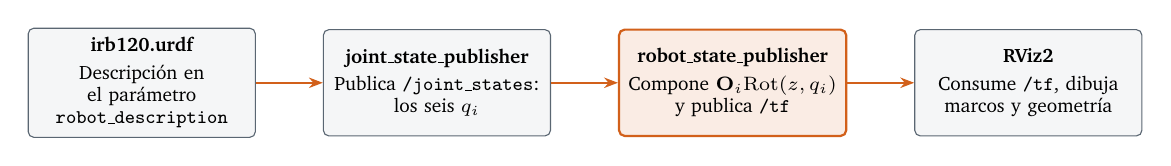
\begin{tikzpicture}[
  nodo/.style={draw=gris,fill=fondocodigo,rounded corners=2pt,
               minimum height=1.35cm,text width=2.65cm,align=center,
               font=\scriptsize},
  destacado/.style={nodo,fill=naranja!12,draw=naranja,thick},
  flecha/.style={-{Stealth[length=5pt]},draw=naranja,thick}
]
\node[nodo] (urdf) {\textbf{irb120.urdf}\\[2pt]Descripción en el parámetro \texttt{robot\_description}};
\node[nodo,right=0.85cm of urdf] (jsp) {\textbf{joint\_state\_publisher}\\[2pt]Publica \texttt{/joint\_states}: los seis $q_i$};
\node[destacado,right=0.85cm of jsp] (rsp) {\textbf{robot\_state\_publisher}\\[2pt]Compone $\mat{O}_i\mathrm{Rot}(z,q_i)$ y publica \texttt{/tf}};
\node[nodo,right=0.85cm of rsp] (rviz) {\textbf{RViz2}\\[2pt]Consume \texttt{/tf}, dibuja marcos y geometría};
\draw[flecha] (urdf) -- (jsp);
\draw[flecha] (jsp) -- (rsp);
\draw[flecha] (rsp) -- (rviz);
\end{tikzpicture}
\caption{Cadena de responsabilidad entre los nodos de ROS 2. El nodo
destacado es el único que realiza composición de transformaciones.}
\label{fig:nodos}
\end{figure}

\subsection{Selección de la distribución}

El listado de materiales del proyecto especifica Ubuntu 24.04 junto con
ROS Noetic o Humble. Esa combinación no es realizable: Noetic está
soportado únicamente sobre Ubuntu 20.04 y Humble sobre Ubuntu 22.04.

Se optó por respetar el sistema operativo indicado en el enunciado y
adoptar \textbf{ROS 2 Jazzy Jalisco}, que es la distribución de soporte
extendido oficialmente asociada a Ubuntu 24.04. La discrepancia se
documenta explícitamente en el repositorio.

\subsection{Árbol cinemático resultante}

La validación sintáctica mediante \texttt{check\_urdf} produce el árbol
de la figura~\ref{fig:arbol}, confirmando una cadena continua sin ramas
accidentales.

\begin{figure}[h]
\centering
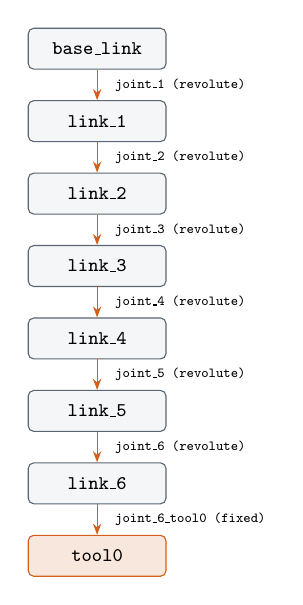
\begin{tikzpicture}[
  every node/.style={font=\scriptsize\ttfamily},
  eslabon/.style={draw=gris,fill=fondocodigo,rounded corners=2pt,
                  minimum width=1.75cm,minimum height=0.52cm},
  brida/.style={eslabon,fill=naranja!15,draw=naranja},
  union/.style={-{Stealth[length=4pt]},draw=naranja}
]
\foreach \i/\n [count=\c from 0] in
  {0/base\_link,1/link\_1,2/link\_2,3/link\_3,4/link\_4,5/link\_5,6/link\_6} {
  \node[eslabon] (l\i) at (0, -0.92*\c) {\n};
}
\node[brida] (l7) at (0,-0.92*7) {tool0};
\foreach \a/\b/\j in {0/1/joint\_1,1/2/joint\_2,2/3/joint\_3,3/4/joint\_4,
                      4/5/joint\_5,5/6/joint\_6} {
  \draw[union] (l\a) -- node[right=3pt,font=\tiny\ttfamily]{\j\ (revolute)} (l\b);
}
\draw[union] (l6) -- node[right=3pt,font=\tiny\ttfamily]{joint\_6\_tool0 (fixed)} (l7);
\end{tikzpicture}
\caption{Árbol cinemático verificado. Cada eslabón posee exactamente un
padre; la brida se une mediante una junta fija.}
\label{fig:arbol}
\end{figure}

%=======================================================================
\section{Validación experimental}
\label{sec:validacion}

\subsection{Pruebas de juntas individuales}

Como control previo al barrido estadístico se movió cada junta
$0{,}5$~rad manteniendo las cinco restantes en cero
(cuadro~\ref{tab:juntas} y figura~\ref{fig:juntas}).

\begin{table}[h]
\centering
\caption{Desplazamiento de \texttt{tool0} al accionar cada junta
individualmente}
\label{tab:juntas}
\small
\begin{tabular}{@{}clll@{}}
\toprule
\textbf{Junta} & \textbf{Posición resultante [m]} & \textbf{$\|\Delta\|$ [m]} & \textbf{Observación} \\
\midrule
J1 & $[0{,}32822,\;0{,}17931,\;0{,}63000]$ & 0,17931 & $z$ y radio conservados \\
J2 & $[0{,}49122,\;0{,}00000,\;0{,}40907]$ & 0,25937 & Movimiento en el plano $xz$ \\
J3 & $[0{,}36178,\;0{,}00000,\;0{,}44213]$ & 0,18795 & Menor brazo de palanca \\
J4 & $[0{,}37400,\;0{,}00000,\;0{,}63000]$ & 0,00000 & Sólo reorienta \\
J5 & $[0{,}36519,\;0{,}00000,\;0{,}59548]$ & 0,03554 & Del orden de $d_6$ \\
J6 & $[0{,}37400,\;0{,}00000,\;0{,}63000]$ & 0,00000 & Sólo reorienta \\
\bottomrule
\end{tabular}
\end{table}

\begin{figure}[h]
\centering
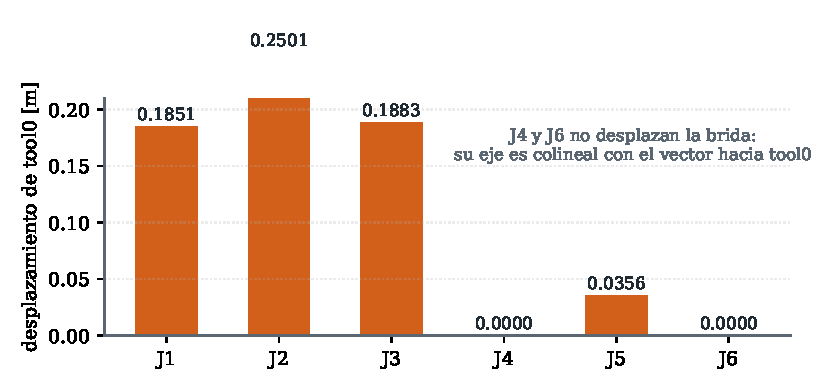
\includegraphics[width=0.78\textwidth]{img/juntas.pdf}
\caption{Desplazamiento del efector al accionar cada junta por separado
desde la configuración cero.}
\label{fig:juntas}
\end{figure}

\begin{nota}
\textbf{Que J4 y J6 no desplacen el efector no constituye un error.} En
ambos casos el eje de rotación es colineal con el vector que une el
origen de la junta con la brida, y una rotación no desplaza los puntos
situados sobre su propio eje. El resultado funciona como verificación
positiva: si J6 desplazara \texttt{tool0}, existiría un error en
$\alpha_5$ o en $d_6$.

J5 sí produce desplazamiento, pero reducido, porque su origen coincide
con el centro de muñeca y únicamente arrastra el saliente
$d_6 = 0{,}072$~m.
\end{nota}

\subsection{Configuraciones de prueba}

\subsubsection*{Prueba A}
\[
\mat{q}^{(A)} = [0{,}3000,\; -0{,}5000,\; 0{,}8000,\; 0{,}2000,\; -0{,}6000,\; 1{,}0000]^{\top}\;\mathrm{rad}
\]
\[
\mat{p}^{(A)} = [0{,}239595,\; 0{,}065661,\; 0{,}525077]^{\top}\;\mathrm{m}
\]
\[
\mat{R}^{(A)} =
\begin{bmatrix}
\phantom{-}0{,}067650 & \phantom{-}0{,}326882 & \phantom{-}0{,}942641\\
-0{,}935061 & -0{,}308747 & \phantom{-}0{,}174171\\
\phantom{-}0{,}347971 & -0{,}893210 & \phantom{-}0{,}284768
\end{bmatrix}
\]

\subsubsection*{Prueba B}
\[
\mat{q}^{(B)} = [-0{,}7854,\; 0{,}5236,\; -0{,}3491,\; 1{,}0472,\; 0{,}7854,\; -1{,}5708]^{\top}\;\mathrm{rad}
\]
\[
\mat{p}^{(B)} = [0{,}377861,\; -0{,}315508,\; 0{,}506423]^{\top}\;\mathrm{m}
\]
\[
\mat{R}^{(B)} =
\begin{bmatrix}
0{,}459870 & \phantom{-}0{,}102799 & \phantom{-}0{,}882016\\
0{,}247237 & -0{,}968823 & -0{,}015990\\
0{,}852874 & \phantom{-}0{,}225420 & -0{,}470948
\end{bmatrix}
\]

En ambos casos la lectura del árbol de transformadas mediante
\texttt{tf2\_echo} coincide con la referencia matemática dentro de la
tolerancia de transporte analizada más adelante.

\subsection{Barrido del espacio articular}

Dos configuraciones puntuales no cubren el espacio de trabajo. Se
implementó por ello un barrido automático que publica configuraciones
aleatorias uniformes dentro de los límites articulares y contrasta la
transformada devuelta por ROS contra la función analítica.

\subsubsection*{Métricas}

\begin{equation}
\varepsilon_p = \left\| \mat{p}_{\mathrm{TF}} - \mat{p}_{\mathrm{ana}} \right\|_2
\qquad [\mathrm{m}]
\end{equation}

\begin{equation}
\varepsilon_R = \left\| \mat{R}_{\mathrm{ana}}^{\top}\,\mat{R}_{\mathrm{TF}} - \mat{I} \right\|_F
\qquad [\text{adimensional}]
\end{equation}

La métrica angular se fundamenta en~\eqref{eq:so3}: dado que la inversa
de una matriz de rotación es su transpuesta, el producto
$\mat{R}_{\mathrm{ana}}^{\top}\mat{R}_{\mathrm{TF}}$ es la identidad si
y sólo si ambas rotaciones coinciden. La norma de Frobenius de su
diferencia con $\mat{I}$ cuantifica el apartamiento.

\begin{nota}
Validar la orientación además de la posición implica verificar los seis
grados de libertad de la pose, y no únicamente los tres de traslación.
\end{nota}

\subsubsection*{Resultados}

\begin{table}[h]
\centering
\caption{Resultados de la validación del árbol TF contra la cinemática
analítica}
\label{tab:resultados}
\small
\begin{tabular}{@{}lrr@{}}
\toprule
\textbf{Métrica} & \textbf{Valor} & \textbf{Umbral} \\
\midrule
Error posicional medio & $1{,}498\times10^{-10}$ m & --- \\
Error posicional máximo & $\mathbf{2{,}459\times10^{-10}}$ \textbf{m} & $1\times10^{-6}$ m \\
Error angular máximo & $1{,}092\times10^{-9}$ & --- \\
Muestras válidas & 501 de 1000 & --- \\
Margen respecto del umbral & $4{,}1\times10^{3}$ veces & --- \\
\bottomrule
\end{tabular}
\end{table}

\begin{figure}[h]
\centering
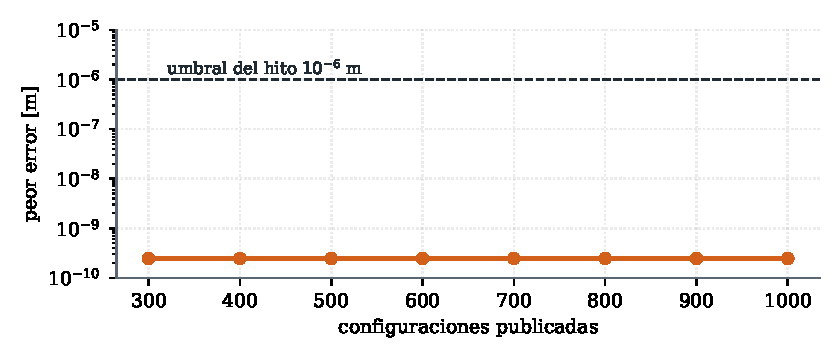
\includegraphics[width=0.85\textwidth]{img/convergencia.pdf}
\caption{Evolución del peor error posicional conforme aumenta el número
de configuraciones evaluadas. El valor se estabiliza a partir de las 300
muestras.}
\label{fig:convergencia}
\end{figure}

La estabilización observada en la figura~\ref{fig:convergencia} indica
que el espacio articular quedó suficientemente explorado: incrementar el
número de muestras no revela casos más desfavorables.

\subsection{Interpretación del orden de magnitud}

Las dos verificaciones realizadas arrojan valores separados por seis
órdenes de magnitud, lo cual merece explicación
(figura~\ref{fig:errores}).

\begin{figure}[h]
\centering
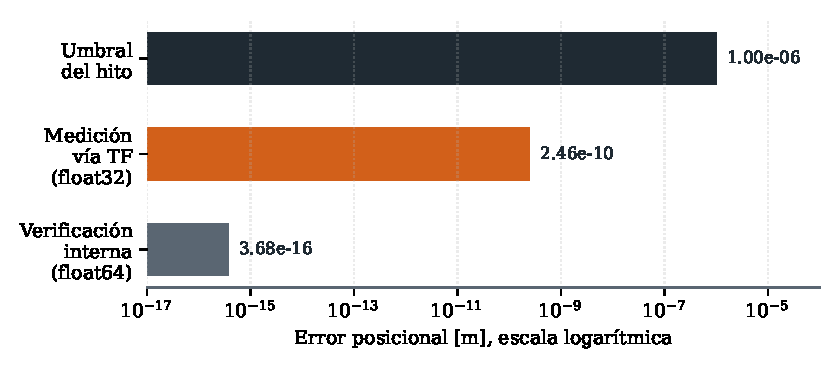
\includegraphics[width=0.85\textwidth]{img/errores.pdf}
\caption{Comparación entre la verificación interna del generador, la
medición a través del árbol TF y el umbral exigido por el hito.}
\label{fig:errores}
\end{figure}

La verificación interna, que no atraviesa la infraestructura de ROS,
arroja $3{,}68\times10^{-16}$~m, valor correspondiente al épsilon de
máquina en doble precisión. La medición a través del árbol de
transformadas arroja $2{,}459\times10^{-10}$~m.

La causa de la diferencia no reside en el modelo sino en el transporte:
ROS transmite las rotaciones como cuaterniones en precisión simple
(\texttt{float32}), cuyo épsilon vale aproximadamente
$1{,}2\times10^{-7}$. La conversión matriz~$\to$~cuaternión~$\to$~matriz,
propagada a lo largo de seis juntas, deja el residuo observado.

\begin{nota}
En consecuencia, lo que la validación mide a través de TF es
\textbf{la precisión del transporte de ROS}, no la del modelo
cinemático. Este último es exacto hasta el límite de la representación
en doble precisión. La distinción explica además por qué el umbral
exigido por el hito es $10^{-6}$~m y no un valor más estricto: ninguna
implementación podría superarlo por medio de TF.
\end{nota}

%=======================================================================
\section{Incidencias detectadas durante el desarrollo}

Se documentan las discrepancias encontradas, junto con su diagnóstico y
corrección. Ninguna de ellas estaba prevista en el enunciado.

\subsection{Conflicto entre publicadores de estado articular}

\textbf{Síntoma.} El procedimiento de validación reportaba un error
posicional máximo de $1{,}110$~m, del orden del alcance del
manipulador. La pose analítica no guardaba relación con la leída del
árbol de transformadas.

\textbf{Diagnóstico.} El nodo \texttt{joint\_state\_publisher}
permanecía activo publicando $\mat{q} = \mat{0}$ de forma continua. Cada
configuración emitida por el validador era sobrescrita antes de que el
árbol se recompusiera, de modo que se comparaba la cinemática analítica
de una configuración aleatoria contra la transformada correspondiente a
la configuración nula.

\textbf{Corrección.} Se separaron ambos comportamientos mediante un
argumento del archivo de lanzamiento. Con \texttt{gui:=true} se activa
la interfaz de deslizadores para la demostración interactiva; con
\texttt{gui:=false} no se instancia ningún publicador de estado
articular, dejando el canal disponible para el validador. Se incorporó
además una comprobación que cuenta los publicadores del tópico y
advierte si existe más de uno.

\subsection{Desfase temporal en la lectura del árbol de transformadas}

\textbf{Síntoma.} Eliminado el conflicto anterior, el error persistía en
el orden de $1{,}217$~m y variaba entre ejecuciones. El error medio
—$0{,}361$~m— correspondía aproximadamente a la distancia esperada entre
dos poses aleatorias distintas.

\textbf{Diagnóstico.} El validador publicaba la configuración, aguardaba
un intervalo fijo de 10~ms y consultaba el árbol mediante
\texttt{lookup\_transform} con marca temporal nula, que devuelve
\emph{la última transformada disponible}. Dado que
\texttt{robot\_state\_publisher} aún no había procesado el mensaje
nuevo, se obtenía la pose correspondiente a la configuración
\emph{anterior}: se comparaba la analítica de $\mat{q}^{(k)}$ contra la
transformada de $\mat{q}^{(k-1)}$.

\textbf{Corrección.} Se sustituyó la espera fija por una sincronización
basada en marcas temporales. Cada mensaje de estado articular se sella
con la hora de emisión, y la lectura se repite hasta que la marca
temporal de la transformada alcanza o supera la del mensaje publicado.

\begin{lstlisting}[language=Python,caption={Sincronización por marca
temporal}]
def leer_tf_sincronizado(self, t_pub_ns, timeout=2.0):
    """
    Relee hasta que la marca de tiempo de la transformada alcanza a la
    del JointState enviado. Asi se garantiza que la pose leida no es
    la de la configuracion anterior.
    """
    fin = time.time() + timeout
    while time.time() < fin:
        rclpy.spin_once(self, timeout_sec=0.005)
        try:
            t = self.buffer.lookup_transform(
                "base_link", "tool0", rclpy.time.Time())
        except Exception:
            continue
        if stamp_a_ns(t.header.stamp) < t_pub_ns:
            continue          # todavia es la pose vieja
        tr, ro = t.transform.translation, t.transform.rotation
        return (np.array([tr.x, tr.y, tr.z]),
                quat_to_matrix(ro.x, ro.y, ro.z, ro.w))
    return None
\end{lstlisting}

Si el tiempo de espera expira, la muestra se \textbf{descarta} en lugar
de contaminar el promedio. Esto explica las 499 lecturas perdidas sobre
1000: no constituyen mediciones erróneas, sino muestras cuya
sincronización no pudo garantizarse. Descartarlas es metodológicamente
más riguroso que incorporarlas.

\subsection{Singularidad en la conversión a ángulos rpy}

\textbf{Síntoma.} La extracción de ángulos \emph{roll-pitch-yaw} del
origen de \texttt{joint\_2} producía valores indefinidos.

\textbf{Diagnóstico.} La matriz correspondiente presenta $R_{31} = 1$, y
la fórmula habitual divide por $\cos\vartheta$, nulo en ese punto. Es el
bloqueo de cardán analizado en la sección~\ref{sec:gimbal}.

\textbf{Corrección.} Tratamiento explícito de la rama degenerada, con
verificación del resultado contra la matriz original y contra la
descripción redactada manualmente.

\subsection{Instalación de directorios de datos}

\textbf{Síntoma.} El paquete compilaba sin advertencias, el árbol de
transformadas se construía correctamente, pero el visualizador no
representaba geometría alguna.

\textbf{Diagnóstico.} El archivo \texttt{CMakeLists.txt} no instalaba
los directorios \texttt{urdf/}, \texttt{meshes/} y \texttt{launch/} en
\texttt{share/}, de modo que las rutas del esquema \texttt{package://}
no resolvían.

\textbf{Corrección.} Incorporación del bloque
\texttt{install(DIRECTORY ...)}. Se destaca por tratarse de un
\textbf{fallo silencioso}: ninguna herramienta emite diagnóstico.

%=======================================================================
\section{Gestión del repositorio}

El proyecto exige un historial de versiones que refleje el proceso real
de trabajo, penalizando las incorporaciones masivas al final del
período.

\begin{table}[h]
\centering
\caption{Historial de contribuciones}
\label{tab:commits}
\small
\begin{tabular}{@{}lll@{}}
\toprule
\textbf{Identificador} & \textbf{Tipo} & \textbf{Descripción} \\
\midrule
\texttt{694189b} & \texttt{chore} & Estructura inicial del paquete \\
\texttt{ee4632e} & \texttt{feat} & Cinemática directa D--H \\
\texttt{5a3051d} & \texttt{feat} & URDF manual y generador derivado \\
\texttt{3adc549} & \texttt{test} & Validación TF contra analítica \\
\texttt{6d19d49} & \texttt{docs} & Documentación del repositorio \\
\texttt{3abc849} & \texttt{docs} & Material demostrativo \\
\texttt{e077c6c} & \texttt{feat} & Geometría por primitivas \\
\bottomrule
\end{tabular}
\end{table}

Se emplea el convenio \emph{Conventional Commits}, cuyos prefijos
permiten generar automáticamente un registro de cambios y rastrear qué
contribución introdujo cada modificación cinemática. La estructura de
ramas comprende \texttt{main} para los estados entregados y \texttt{dev}
para la integración. La entrega se identifica mediante la etiqueta
\texttt{v1.0-hito1}.

%=======================================================================
\section{Conclusiones}

\begin{enumerate}[leftmargin=*]

\item Se construyó un gemelo digital cinemático del ABB IRB 120 cuya
descripción URDF reproduce la cinemática directa analítica con un error
posicional máximo de $2{,}459\times10^{-10}$~m sobre 501 configuraciones
válidas, cuatro mil veces por debajo del umbral exigido, con validación
simultánea de la orientación.

\item La contribución metodológica principal consiste en haber
establecido una relación algebraica cerrada entre ambos formalismos,
ecuación~\eqref{eq:puente}. Los atributos \texttt{origin} del URDF no
fueron ajustados visualmente sino derivados, de modo que la coincidencia
con el producto $\T{0}{6}$ no es una aproximación afortunada sino una
consecuencia estructural de la construcción.

\item La validación se sostiene sobre tres pruebas mutuamente
independientes: la predicción de la pose en configuración cero por suma
de cotas del manual, que verifica la transcripción de la tabla sin
ejecutar código; la equivalencia demostrada entre la descripción
redactada manualmente y la generada programáticamente, que descarta
errores de transcripción; y el barrido aleatorio del espacio articular
contra el árbol de transformadas.

\item Se estableció que la verificación en $\mat{q} = \mat{0}$ es
necesaria pero insuficiente, por tratarse de un caso degenerado en el
que los eslabones se alinean con sólo dos ejes del marco base.

\item Se determinó que el error medido a través del árbol de
transformadas cuantifica la precisión del transporte de ROS
—cuaterniones en precisión simple— y no la del modelo cinemático, cuya
exactitud alcanza el épsilon de la doble precisión.

\item Se documentaron cuatro incidencias técnicas, dos de ellas con
errores superiores a un metro, junto con su diagnóstico y corrección. Se
considera que un resultado correcto sin trazabilidad del proceso que
condujo a él no sería defendible.

\item El modelo validado constituye la entrada directa del resolvedor de
cinemática inversa por desacoplamiento de Pieper correspondiente al
Hito 2, sin necesidad de reelaboración.

\end{enumerate}

%=======================================================================
\section{Trabajo futuro}

\begin{itemize}[leftmargin=*]
\item Incorporación de mallas tridimensionales de los eslabones para el
modelo visual de alta fidelidad.
\item Diseño en SolidWorks de la pinza neumática, acoplada como eslabón
hijo de \texttt{tool0} mediante junta fija.
\item Incorporación de propiedades inerciales que habiliten la
simulación dinámica en Gazebo.
\item Hito 2: cinemática inversa por desacoplamiento de Pieper y
perfiles de velocidad LSPB.
\end{itemize}

%=======================================================================
\appendix
\section{Comandos de reproducción}

\begin{lstlisting}[language=bash,caption={Secuencia completa de
verificación}]
# Compilacion
cd ~/ros2_ws
colcon build --packages-select irb120_description
source install/setup.bash

# 1. Cinematica analitica: p(q=0) = [0.374, 0, 0.630] m
cd src/irb120_description/scripts
python3 fk_irb120.py

# 2. Generacion del URDF y verificacion interna de la cadena
python3 generate_urdf.py

# 3. Equivalencia entre descripcion manual y derivada
python3 compare_urdf.py

# 4. Validacion sintactica y arbol cinematico
check_urdf ../urdf/irb120.urdf

# 5. Visualizacion interactiva
ros2 launch irb120_description display.launch.py
ros2 run tf2_ros tf2_echo base_link tool0     # en otra terminal

# 6. Validacion TF contra analitica
ros2 launch irb120_description display.launch.py gui:=false
python3 validate_tf.py 1000                   # en otra terminal

# 7. Comprobacion con la descripcion escrita a mano
ros2 launch irb120_description display.launch.py modelo:=irb120_manual
\end{lstlisting}

\section{Estructura del repositorio}

\begin{lstlisting}[caption={Organización de archivos}]
irb120_description/
|- urdf/
|  |- irb120_manual.urdf     escrito a mano, procedencia documentada
|  `- irb120.urdf            generado por script
|- scripts/
|  |- fk_irb120.py           cinematica directa, solo NumPy
|  |- generate_urdf.py       derivacion D-H -> URDF
|  |- compare_urdf.py        equivalencia manual vs. derivado
|  |- validate_tf.py         validacion contra el arbol TF
|  `- add_visuals.py         geometria por primitivas
|- launch/display.launch.py
|- rviz/irb120.rviz
|- docs/validacion_hito1.txt evidencia numerica
|- CMakeLists.txt
|- package.xml
`- README.md
\end{lstlisting}

%=======================================================================
\begin{thebibliography}{9}

\bibitem{siciliano}
Siciliano, B., Sciavicco, L., Villani, L., Oriolo, G. (2009).
\emph{Robotics: Modelling, Planning and Control}. Springer-Verlag London.

\bibitem{spong}
Spong, M. W., Hutchinson, S., Vidyasagar, M. (2006).
\emph{Robot Modeling and Control}. John Wiley \& Sons.

\bibitem{craig}
Craig, J. J. (2005). \emph{Introduction to Robotics: Mechanics and
Control}. 3ª edición. Pearson Prentice Hall.

\bibitem{truclam}
Truc, L. N., Lam, N. T. (2020). Parametrización Denavit--Hartenberg del
manipulador ABB IRB 120.

\bibitem{denavit}
Denavit, J., Hartenberg, R. S. (1955). A kinematic notation for
lower-pair mechanisms based on matrices. \emph{Journal of Applied
Mechanics}, 22, 215--221.

\bibitem{pieper}
Pieper, D. L. (1968). \emph{The Kinematics of Manipulators Under
Computer Control}. Tesis doctoral, Universidad de Stanford.

\bibitem{abb}
ABB Robotics. \emph{Product Specification IRB 120}. Documento técnico
del fabricante.

\bibitem{ros}
Open Robotics. \emph{ROS 2 Documentation: Jazzy Jalisco}.
\url{https://docs.ros.org}

\bibitem{urdf}
Open Robotics. \emph{URDF XML Specification}.
\url{http://wiki.ros.org/urdf/XML}

\end{thebibliography}

\end{document}
